\documentclass[]{article}
\usepackage{lmodern}
\usepackage{amssymb,amsmath}
\usepackage{ifxetex,ifluatex}
\usepackage{fixltx2e} % provides \textsubscript
\ifnum 0\ifxetex 1\fi\ifluatex 1\fi=0 % if pdftex
  \usepackage[T1]{fontenc}
  \usepackage[utf8]{inputenc}
\else % if luatex or xelatex
  \ifxetex
    \usepackage{mathspec}
  \else
    \usepackage{fontspec}
  \fi
  \defaultfontfeatures{Ligatures=TeX,Scale=MatchLowercase}
\fi
% use upquote if available, for straight quotes in verbatim environments
\IfFileExists{upquote.sty}{\usepackage{upquote}}{}
% use microtype if available
\IfFileExists{microtype.sty}{%
\usepackage{microtype}
\UseMicrotypeSet[protrusion]{basicmath} % disable protrusion for tt fonts
}{}
\usepackage{hyperref}
\hypersetup{unicode=true,
            pdfborder={0 0 0},
            breaklinks=true}
\urlstyle{same}  % don't use monospace font for urls
\usepackage{graphicx,grffile}
\makeatletter
\def\maxwidth{\ifdim\Gin@nat@width>\linewidth\linewidth\else\Gin@nat@width\fi}
\def\maxheight{\ifdim\Gin@nat@height>\textheight\textheight\else\Gin@nat@height\fi}
\makeatother
% Scale images if necessary, so that they will not overflow the page
% margins by default, and it is still possible to overwrite the defaults
% using explicit options in \includegraphics[width, height, ...]{}
\setkeys{Gin}{width=17cm,height=\maxheight,keepaspectratio}
\IfFileExists{parskip.sty}{%
\usepackage{parskip}
}{% else
\setlength{\parindent}{0pt}
\setlength{\parskip}{6pt plus 2pt minus 1pt}
}
\setlength{\emergencystretch}{3em}  % prevent overfull lines
\providecommand{\tightlist}{%
  \setlength{\itemsep}{0pt}\setlength{\parskip}{0pt}}
\setcounter{secnumdepth}{0}
% Redefines (sub)paragraphs to behave more like sections
\ifx\paragraph\undefined\else
\let\oldparagraph\paragraph
\renewcommand{\paragraph}[1]{\oldparagraph{#1}\mbox{}}
\fi
\ifx\subparagraph\undefined\else
\let\oldsubparagraph\subparagraph
\renewcommand{\subparagraph}[1]{\oldsubparagraph{#1}\mbox{}}
\fi

\date{}

\begin{document}

\subsection{Title}\label{title}

Simulations of Silicon-on-Insulator Channel-Waveguide Electrooptical 2 ×
2 Switches and 1 × 1 Modulators Using a \(\mathrm{Ge_2 Sb_2 Te_5}\)
Self-Holding Layer

\subsection{Authors}\label{authors}

\begin{itemize}
\tightlist
\item
  Haibo Liang
\item
  Richard Soref
\item
  Jianwei Mu
\item
  Arka Majumdar
\item
  Xun Li
\item
  Wei-Ping Huang
\end{itemize}

\subsection{Abstract}\label{abstract}

2 × 2 switches and 1 × 1 loss modulators based upon GST-embedded SOI
channel waveguides

10-nm GST film sandwiched between doped-Si waveguide strips

1.3 to 2.1-\(\mathrm{\mu m}\) wavelength range

2 × 2 Mach--Zehnder and directional coupler switches

1 × 1 EO waveguide has application as a variable optical attenuator and
as a digital modulator for 1.3-2.1 \(\mathrm{\mu m}\)

\subsection{Highlight}\label{highlight}

The design presented here is new in two ways:\\
(1) the thin film is placed midway in the body of the waveguide where it
has a much stronger effect upon the mode indices;\\
(2) the phase change---rather than being optically triggered---is
electrically induced. (3)utilize both the electro-refraction (ER) and
the electro- absorption (EA) component of the induced phase change\\
\centerline{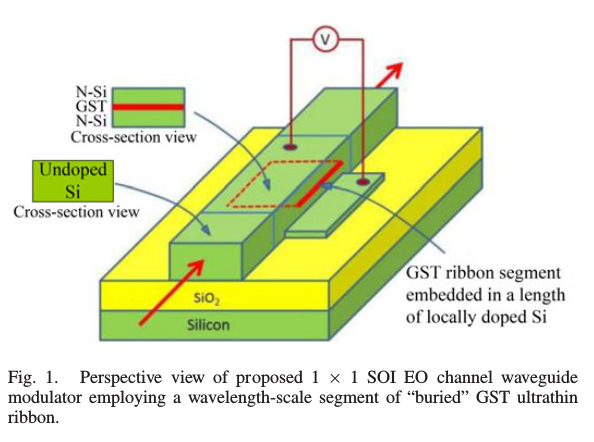
\includegraphics[width=10cm]{image/004_01.png}} \centerline{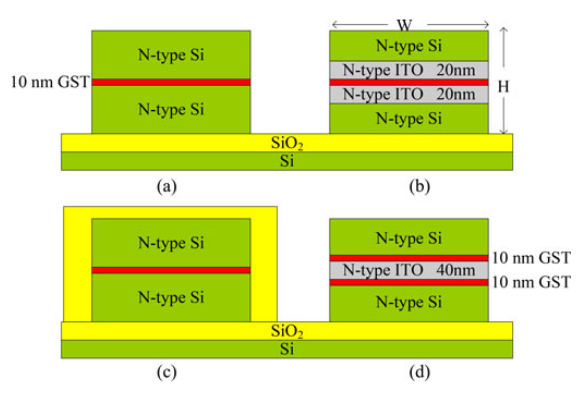
\includegraphics[width=10cm]{image/004_02.png}}

Unexpectedly, the TE-polarized light is particularly sensitive to the
induced change of GST complex index \(\mathrm{\Delta n + i\,\Delta k}\),
more so than in TM. Unexpectedly, the ratio
\(\mathrm{{\Delta n}/{\Delta k}}\) is consistently higher in TM than TE.
The loss suppression in TM indicates that ER dominates in TM. Thus, with
the anti-slot, TM is more favorable for low-loss 2 × 2 switching,
whereas TE is the most natural mode polarization for 1 × 1 EA
applications.

\newpage
\paragraph{ELECTRICALLY INDUCED PHASE
CHANGE}\label{electrically-induced-phase-change}

In detail, the recrystallization requires an applied set voltage pulse
of 100-ns duration that induces temperature rise above \textbf{413 K}
but below \textbf{819 K} (the melting point).

As for the changing process from crystalline to amorphous state, a
shorter reset voltage pulse of typically 1 to 10 ns duration is
employed, and there the GST film temperature must be raised above the
melting point(above the \textbf{891 K} as desired) and then quenched
rapidly by the pulse falling to zero in \textless{} 1 ns.

The voltages (5V and 15V) that we applied in both simulations might be
considered as ``\emph{relatively high}''; however, this is a trade-off
we are willing tomake to achieve optimum optical performances in the
coming sections.

\paragraph{PERFORMANCE GUIDELINES FOR 2 × 2
SWITCHES}\label{performance-guidelines-for-2-2-switches}

\centerline{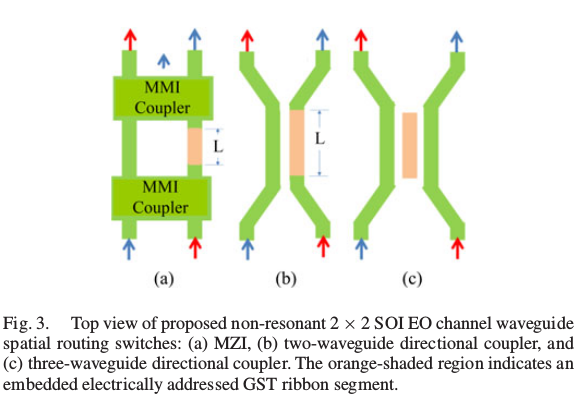
\includegraphics[width=10cm]{image/004_03.png}}
The GST indices are written for the amorphous phase
\(\mathrm{n_{am} + i\,k_{am} = n_1 + i\,k_1}\) , and for the crystalline
phase \(\mathrm{n_{cr} + i\,k_{cr} = n_2 + i\,k_2}\) , while the channel
waveguide has a mode effective index in each state written as
\(\mathrm{n_{1e} + i\,k_{1e}}\) and \(\mathrm{n_{2e} + i\,k_{2e}}\) .
Looking at the extinction coefficient k, let us denote \(\alpha\) as the
absorption loss of the waveguide in decibel per micrometer in each
state, \(\mathrm{\alpha = 4.34(4\pi k/\lambda}\)). The IL of an
amorphous active waveguide of length L is proportional to the product
\(\alpha\)L, that is \emph{IL} (dB) =
\(\mathrm{4.34(4\pi k_{1e} L/\lambda}\)) and the crystalline-phase loss
is \(\mathrm{4.34(4\pi k_{2e} L/\lambda}\)). The extinction ratio of a
loss modulator discussed below is then \emph{ER} (dB) =
\(\mathrm{(k_{2e} – k_{1e})(4.34)(4\pi L/\lambda})\).

Loss modulation utilizes EA, while ER is mostly neglected: 2 × 2
switching relies upon ER, with additional requirements that: (1) ER
\textgreater{}\textgreater{} EA, and (2) absorption loss in the initial
cross state is low.

In switches, it is the product of the phase factor \(\Delta \beta\) with
L, that affects the transfer of light from the input guide to the output
guide, where
\(\mathrm{\Delta \beta L = (2\pi/\lambda)(n_{2e} – n_{1e})}\). Values of
\(\Delta \beta\)L from 3 to 18 are required, depending upon the switch
geometry and upon whether the device is resonant or non-resonant.
Specifically the Mach--Zehnder interferometer (MZI) requires
\(\Delta \beta\)L = \(\pi\) rad, while the two-waveguide directional
coupler needs \(\Delta \beta\)L = 5.4 rad, and the three-waveguide
directional coupler requires \(\Delta \beta\)L = 18 rad.\\
To minimize \emph{IL} and crosstalk (\emph{CT}) in both switching
states, we generally desire
\(\mathrm{n_{2e} – n_{1e} >> k_{2e} – k_{1e}}\) with the ratio
\(\mathrm{\rho = (n_{2e} – n_{1e})/(k_{2e} – k_{1e})}\) being as high as
possible.

\paragraph{RESULTS OF NUMERICAL
SIMULATIONS}\label{results-of-numerical-simulations}

\textbf{PREDICTED 2 × 2 SWITCHING PERFORMANCE:}\\
\centerline{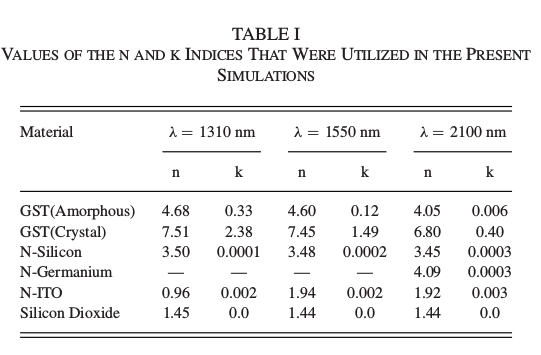
\includegraphics[width=8cm]{image/004_04.png}}\\
\centerline{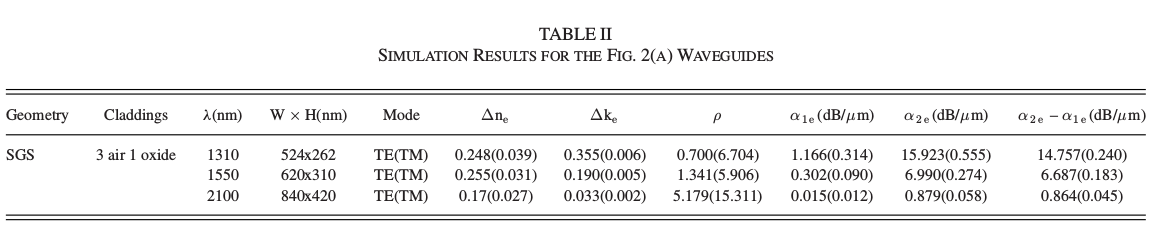
\includegraphics{image/004_05.png}}\\
\centerline{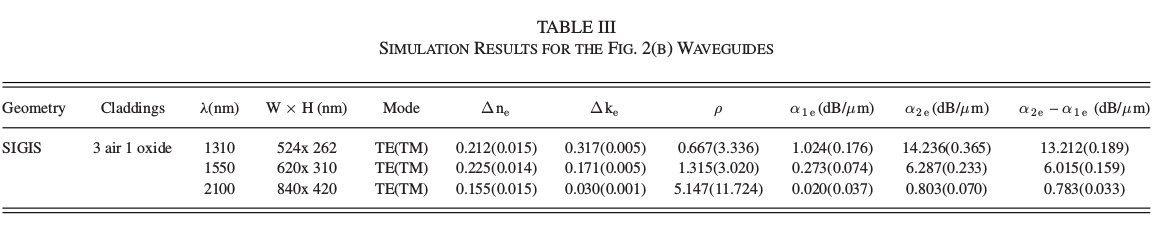
\includegraphics{image/004_06.png}}\\
\centerline{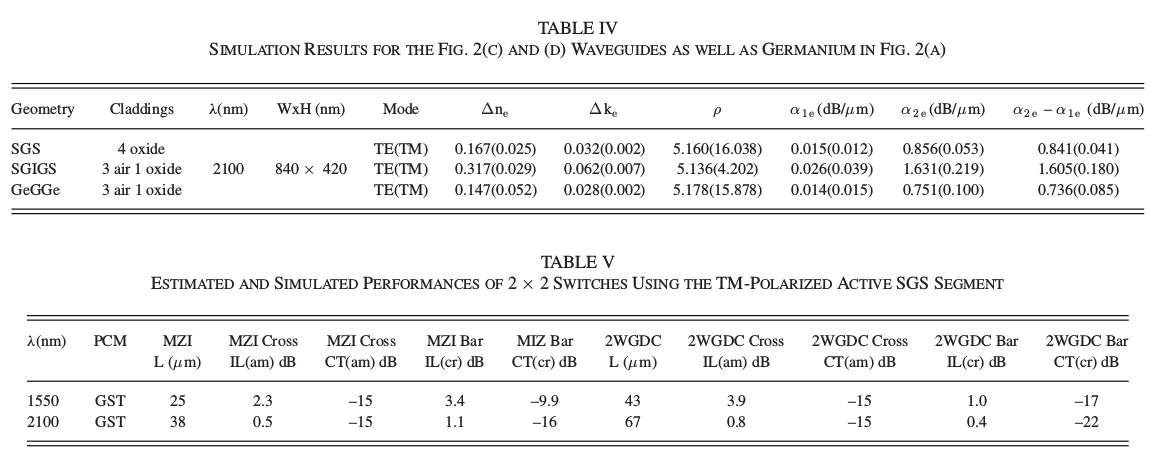
\includegraphics{image/004_07.png}}\\

\textbf{PREDICTED 1 × 1 MODULATOR AND VOA PERFORMANCE:}\\
\centerline{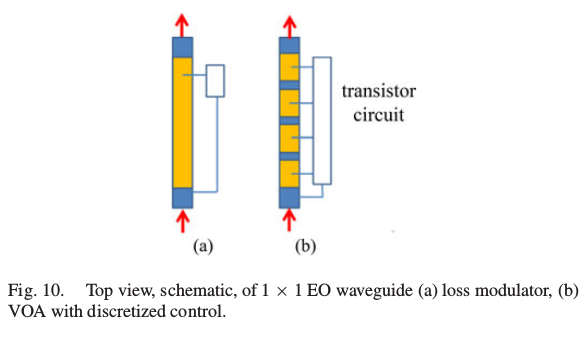
\includegraphics[width=10cm]{image/004_08.png}}

\subsection{Related work}\label{related-work}

\begin{itemize}
\tightlist
\item
  Ultra-small self-holding, optical gate switch using
  \(\mathrm{Ge_2 Sb_2 Te_5}\) with a multi-mode Si waveguide
\item
  Small-sized Mach-Zehnder interferometer optical switch using thin film
  \(\mathrm{Ge_2 Sb_2 Te_5}\) phase-change material
\item
  Mid-infrared 2 × 2 electro-optical switching by silicon and germanium
  three-waveguide and four-waveguide directional couplers using
  free-carrier injection
\item
  An all-optical non-volatile, bidirectional, phase-change meta-switch
\item
  Self-holding optical switch using phase-change material for energy
  efficient photonic network
\end{itemize}

\end{document}
